% =====================================================================
% SkyNest · Hito 2: secciones 4 a 7
% Los resultados del experimento se leen de resultados/ (bench/experimento.py).
% Las cifras citadas en el texto corresponden a la corrida oficial del 14/11/2026
% (Apple M1, PostgreSQL 14.25) guardada en resultados/.
% =====================================================================

\newpage
\section{Implementación de la base de datos}

La base se implementó en PostgreSQL 14 con scripts SQL numerados que se ejecutan en orden. Todos se pueden volver a ejecutar sin errores y cada uno tiene un script de prueba que deja la base como estaba (transacción con \texttt{ROLLBACK}).

\begin{table}[H]
\centering\small
\caption{Scripts de la implementación}
\label{tab:scripts}
\begin{tabularx}{\linewidth}{@{}>{\raggedright\arraybackslash}p{5cm}>{\raggedright\arraybackslash}X@{}}
\toprule
Script & Contenido \\
\midrule
\archivo{sql/01_schema.sql} & esquemas \texttt{skynest} y \texttt{reportes}; 16 tablas con PK, FK, UNIQUE, CHECK y EXCLUDE (sección~\ref{sec:tablas}) \\
\archivo{sql/02_datos_reales.sql} & distritos, modelos de drone y nests reales (sección~\ref{sec:carga}) \\
\archivo{gen/generar.py} & generador de datos sintéticos coherentes y carga con \texttt{COPY} \\
\archivo{sql/03_triggers.sql} & 17 triggers: restricciones (i)--(x) y automatización de estados \\
\archivo{sql/04_procedimientos.sql} & 9 procedimientos del flujo de un envío \\
\archivo{sql/05_vistas.sql} & 9 vistas de usuario y la función de rastreo \\
\archivo{sql/06_roles.sql} & 7 roles con privilegios mínimos \\
\archivo{sql/07_consultas.sql}\newline\archivo{sql/08_indices.sql} & consultas y planes de índices del experimento \\
\archivo{gen/construir_bases.sh} & construye las 4 bases, las verifica y genera los 4 dumps \\
\archivo{bench/experimento.py} & ejecuta el experimento y genera tablas y gráficos \\
\bottomrule
\end{tabularx}
\end{table}

% ---------------------------------------------------------------------
\subsection{Creación de Tablas en PostgreSQL}
\label{sec:tablas}

\archivo{sql/01_schema.sql} traduce el diccionario de datos de la sección 3.3 sin cambios de nombres, tipos ni nulos, para que el modelo físico coincida con el relacional. Las decisiones de implementación fueron:

\begin{enumerate}[label=\arabic*.]
\item \textbf{Restricciones con nombre} (\texttt{pk\_}, \texttt{fk\_}, \texttt{uq\_}, \texttt{ck\_}, \texttt{ex\_}). Así, cada error indica qué regla se violó, por ejemplo \texttt{violates check constraint "ck\_telemetria\_carga"}.
\item \textbf{Las reglas que solo dependen de una fila se implementaron como CHECK}, no como trigger: los dominios de R18 y las dos condiciones de R19. Además se agregaron tres CHECK que implementan reglas ya existentes:
  \begin{itemize}
  \item \texttt{ck\_bateria\_salud\_estado}: una batería con \at{salud\_pct} $< 70$ no puede estar \at{operativa} (R12).
  \item \texttt{ck\_vuelo\_estado\_tiempos}: el estado del vuelo es coherente con sus horarios. Un vuelo \at{programado} o \at{cancelado} no tiene despegue; uno \at{completado} tiene despegue y aterrizaje.
  \item \texttt{ck\_paquete\_coordenadas}: la latitud y la longitud de destino se registran juntas o faltan juntas.
  \end{itemize}
\item \textbf{R12 (una batería no puede estar en dos vuelos a la vez) con una restricción \texttt{EXCLUDE}} sobre el par (batería, intervalo del vuelo), que requiere la extensión \texttt{btree\_gist}. Solo se aplica cuando el vuelo ya tiene despegue y aterrizaje:
\begin{lstlisting}[style=sql]
CONSTRAINT ex_vuelo_bateria_solape EXCLUDE USING gist (
    id_bateria WITH =,
    tsrange(despegue, aterrizaje) WITH &&
) WHERE (despegue IS NOT NULL AND aterrizaje IS NOT NULL)
\end{lstlisting}
\item \textbf{ON DELETE}: \texttt{CASCADE} en las entidades débiles (\tb{punto\_ruta}, \tb{telemetria\_bateria}) y en las subclases de cliente; en las demás FK, el valor por defecto (\texttt{NO ACTION}), que impide, por ejemplo, borrar un drone que ya voló.
\item \textbf{Sin índices adicionales}: solo existen los que PostgreSQL crea por sí mismo para PRIMARY KEY, UNIQUE y EXCLUDE. Las FOREIGN KEY no crean índice en PostgreSQL. Los índices del experimento se definen aparte (sección~\ref{sec:planes}).
\end{enumerate}

\archivo{sql/01_schema_prueba.sql} inserta un envío válido de punta a punta e intenta 13 violaciones (PK, UNIQUE, FK, CHECK y EXCLUDE). Las 13 son rechazadas con la restricción esperada.

% ---------------------------------------------------------------------
\subsubsection{Esquemas}
\label{sec:esquemas}

Un esquema es una carpeta con nombre dentro de la base: agrupa tablas, vistas y funciones, y se le pueden dar permisos como a un todo. La base \texttt{skynest\_<escala>} se organizó en dos esquemas:

\begin{table}[H]
\centering\small
\caption{Esquemas de la base}
\label{tab:esquemas}
\begin{tabular}{l>{\raggedright\arraybackslash}p{6.4cm}>{\raggedright\arraybackslash}p{5cm}}
\toprule
Esquema & Contenido & Quién entra (\texttt{USAGE}) \\
\midrule
\texttt{skynest} & el núcleo: 16 tablas, 12 funciones de trigger y 9 procedimientos & administrador, despachador, operador, técnico, telemetría y cliente \\
\texttt{reportes} & 9 vistas y la función de rastreo (\texttt{fn\_rastrear\_paquete}) & administrador, despachador, operador, técnico, analista y cliente \\
\texttt{public} & solo la extensión \texttt{btree\_gist} & --- \\
\bottomrule
\end{tabular}
\end{table}

La separación tiene dos efectos. Primero, el modelo queda ordenado: lo que se guarda (\texttt{skynest}) está aparte de lo que se consulta para reportar (\texttt{reportes}). Segundo, la seguridad es más simple: el analista recibe \texttt{USAGE} solo sobre \texttt{reportes}, por lo que no puede ni ver los nombres de las tablas del núcleo; si intenta \texttt{SELECT * FROM skynest.paquete}, PostgreSQL responde \texttt{permission denied for schema skynest} antes de revisar permisos de tabla.

Para no escribir el esquema en cada consulta, \archivo{sql/01_schema.sql} fija la ruta de búsqueda por defecto de la base:
\begin{lstlisting}[style=sql]
CREATE SCHEMA skynest;
CREATE SCHEMA reportes;
ALTER DATABASE skynest_1m SET search_path = skynest, reportes, public;
\end{lstlisting}
Así, \texttt{SELECT * FROM vuelo} se resuelve como \texttt{skynest.vuelo} y \texttt{v\_peso\_vuelo} como \texttt{reportes.v\_peso\_vuelo}. Los procedimientos \texttt{SECURITY DEFINER} y la función de rastreo fijan su propio \texttt{search\_path}, para que un usuario no pueda engañarlos creando una tabla con el mismo nombre en otro esquema.

% ---------------------------------------------------------------------
\subsection{Carga de datos}
\label{sec:carga}

\paragraph{Datos reales} (\archivo{sql/02_datos_reales.sql}):
\begin{itemize}
\item \textbf{50 distritos} de Lima Metropolitana (43) y del Callao (7) con su código UBIGEO del INEI. Se consideran restringidos (altitud máxima de 60\,m) Callao, Bellavista y Carmen de la Legua Reynoso, por el Aeropuerto Jorge Chávez, y Lima Cercado, por el Palacio de Gobierno. Es un supuesto del proyecto, no un dato oficial.
\item \textbf{8 modelos de drone} con los valores de sus fichas técnicas públicas: DJI FlyCart 30 y FlyCart 100, Wingcopter 198, Matternet M2 y M3, Zipline P2, Wing Hummingbird y el octocóptero de Manna. Cuando el fabricante no publica la autonomía en minutos, se estimó como alcance / velocidad de crucero.
\item \textbf{30 nests} en avenidas reales de 30 distritos no restringidos, con coordenadas aproximadas; la capacidad total es de 338 drones.
\end{itemize}

\paragraph{Datos sintéticos} (\archivo{gen/generar.py}). La escala $N$ es el \textbf{número de vuelos}, porque el vuelo es el centro del modelo: de él dependen los paquetes y la telemetría. Las demás tablas se derivan de $N$:

\begin{itemize}
\item \textbf{Paquetes}: el número de paquetes de cada vuelo se sortea con $P(0)=4\,\%$, $P(1)=45\,\%$, $P(2)=39\,\%$ y $P(3)=12\,\%$. Los que no caben por peso (R15) se descartan, y se agrega un 2\,\% de paquetes aún sin vuelo. El resultado es de \textbf{1,5 paquetes por vuelo}, la misma proporción del Hito 1 (900\,000 / 600\,000).
\item \textbf{Telemetría}: \textbf{5 lecturas por vuelo} (despegue, tres intermedias y aterrizaje). Es un submuestreo respecto de la lectura cada 5\,s de la sección 1.5.5, porque esa frecuencia daría 180 millones de lecturas en la escala de un millón. Cinco lecturas bastan para calcular el consumo (primera menos última) y detectar sobrecalentamientos (lecturas intermedias).
\item \textbf{Clientes}: uno por cada 15 paquetes (proporción del Hito 1), 75\,\% personas y 25\,\% empresas.
\item \textbf{Tablas maestras fijas} en las cuatro escalas: 300 drones (10 por nest), 900 baterías (3 por drone), 120 operadores (4 por nest), 600 rutas (20 por nest) y sus puntos de ruta.
\end{itemize}

\begin{table}[H]
\centering\small
\caption{Filas por escala (semilla fija 2026: cada ejecución genera los mismos datos)}
\label{tab:filas}
\begin{tabular}{lrrrr}
\toprule
Tabla & 1k & 10k & 100k & 1M \\
\midrule
\tb{vuelo} & 1\,000 & 10\,000 & 100\,000 & 1\,000\,000 \\
\tb{paquete} & 1\,531 & 15\,081 & 150\,219 & 1\,502\,865 \\
\tb{telemetria\_bateria} & 4\,867 & 48\,496 & 484\,933 & 4\,851\,512 \\
\tb{cliente} & 101 & 1\,013 & 10\,133 & 101\,333 \\
\midrule
\multicolumn{5}{l}{Fijas: 600 rutas, 4\,236 puntos de ruta, 300 drones, 900 baterías, 120 operadores,} \\
\multicolumn{5}{l}{\phantom{Fijas: }7\,872 autorizaciones y 32 permisos (trimestrales, uno por distrito restringido)} \\
\bottomrule
\end{tabular}
\end{table}

Los datos se generan respetando todas las reglas, de modo que se cargan sin rechazos:
\begin{itemize}
\item Cada drone solo vuela rutas de su nest (R10) y con alcance suficiente para ida y vuelta con 20\,\% de reserva.
\item El operador es del mismo nest, tiene licencia vigente y autorización para el modelo y el distrito (R11).
\item Los vuelos a distritos restringidos llevan el permiso vigente de ese distrito (R9).
\item Cada drone usa sus 3 baterías por turnos y sus vuelos ocupan franjas de 40 minutos que no se solapan, así que una batería nunca está en dos vuelos a la vez (R12).
\item El distrito del paquete es el destino de la ruta (R14) y el peso del vuelo no supera la carga útil (R15).
\item Las lecturas caen entre el despegue y el aterrizaje (R17).
\end{itemize}

La carga usa \texttt{COPY} con \texttt{session\_replication\_role = replica}, que desactiva los triggers y las FK durante la carga masiva. Los CHECK, PK, UNIQUE y EXCLUDE siguen activos. Como las FK no se validan en ese momento, \archivo{gen/verificar.sql} comprueba después 18 reglas (huérfanos, R2, R6, R9--R12, R14--R17, cobertura de clientes) y en las cuatro escalas da \textbf{0 violaciones}. La escala de un millón se genera en unos 60\,s y se carga con \texttt{COPY} en otros 60\,s (122\,s en total en la plataforma de pruebas); construir las cuatro escalas, con verificación y dumps, toma unos 3,5 minutos.

% ---------------------------------------------------------------------
\subsection{Simulación de Datos Faltantes}

Se simularon los dos tipos de dato faltante previstos en la sección 1.8.1:

\begin{itemize}
\item \textbf{Lecturas perdidas por fallas de señal}: el 3\,\% de los vuelos completados pierde una de sus lecturas intermedias. Estos vuelos tienen 4 lecturas en lugar de 5.
\item \textbf{Paquetes sin coordenadas exactas}: el 5\,\% de los paquetes tiene \at{lat\_destino} y \at{lon\_destino} nulas, permitidas por el diccionario de datos y controladas por \texttt{ck\_paquete\_coordenadas}.
\end{itemize}

\textbf{Tratamiento}:
\begin{itemize}
\item Las consultas de consumo usan la primera y la última lectura \emph{disponibles} de cada vuelo, así que una lectura intermedia perdida no altera el resultado.
\item Las vistas cuentan las lecturas por vuelo (\at{n\_lecturas} en \texttt{v\_historial\_bateria}), lo que permite identificar los vuelos incompletos.
\item Para los paquetes sin coordenadas, la entrega se ubica por la dirección y por el distrito destino, que nunca es nulo.
\end{itemize}

% ---------------------------------------------------------------------
\subsection{Views}

Las vistas exponen los datos derivados que el modelo no almacena (sección 2.3.17) y los reportes de la sección 1.5.2:

\begin{table}[H]
\centering\small
\caption{Vistas de usuario (\archivo{sql/05_vistas.sql})}
\begin{tabular}{lp{9.6cm}}
\toprule
Vista & Uso \\
\midrule
\texttt{v\_seguimiento\_paquete} & estado y vuelo de cada paquete por código de tracking \\
\texttt{v\_peso\_vuelo} & peso total por vuelo frente a la carga útil (no se almacena en \tb{vuelo}) \\
\texttt{v\_historial\_bateria} & uso de cada batería por vuelo: carga inicial y final, consumo y temperatura máxima \\
\texttt{v\_entregas\_nest\_distrito} & paquetes, tasa de éxito y minutos promedio de entrega por nest, distrito y mes \\
\texttt{v\_retrasos\_express} & paquetes express entregados: minutos reales frente a la duración estimada \\
\texttt{v\_consumo\_modelo\_ruta} & consumo de batería en puntos porcentuales por km, por modelo y ruta \\
\texttt{v\_utilizacion\_flota} & vuelos y horas por drone y mes frente al promedio de su modelo \\
\texttt{v\_alertas\_temperatura} & lecturas sobre 60\,\textdegree C con batería, drone y distrito \\
\texttt{v\_licencias\_por\_vencer} & operadores cuya licencia vence en 30 días y sus vuelos programados \\
\bottomrule
\end{tabular}
\end{table}

Para el rol cliente se creó la función \texttt{fn\_rastrear\_paquete(codigo)} (\texttt{SECURITY DEFINER}). El cliente puede consultar un paquete solo si conoce su código de tracking, sin acceso a la vista completa. Ejemplo de vista derivada:

\begin{lstlisting}[style=sql]
CREATE OR REPLACE VIEW v_peso_vuelo AS
SELECT v.id_vuelo, v.estado, m.fabricante || ' ' || m.nombre AS modelo,
       count(p.id_paquete) AS n_paquetes,
       COALESCE(sum(p.peso_kg), 0) AS peso_total_kg, m.carga_util_max_kg,
       round(100 * COALESCE(sum(p.peso_kg), 0) / m.carga_util_max_kg, 1) AS ocupacion_pct
FROM vuelo v
JOIN drone d        ON d.id_drone  = v.id_drone
JOIN modelo_drone m ON m.id_modelo = d.id_modelo
LEFT JOIN paquete p ON p.id_vuelo  = v.id_vuelo
GROUP BY v.id_vuelo, v.estado, m.fabricante, m.nombre, m.carga_util_max_kg;
\end{lstlisting}

% ---------------------------------------------------------------------
\subsection{Procedimientos Almacenados}

Los procedimientos implementan el flujo de un envío de la sección 1.4.2. Reparto de responsabilidades: los procedimientos \emph{deciden} y los triggers \emph{validan}. Por eso, una operación hecha fuera de un procedimiento también queda controlada.

\begin{table}[H]
\centering\small
\caption{Procedimientos almacenados (\archivo{sql/04_procedimientos.sql})}
\begin{tabularx}{\linewidth}{@{}>{\raggedright\arraybackslash}p{5.6cm}>{\raggedright\arraybackslash}X@{}}
\toprule
Procedimiento & Qué hace \\
\midrule
\texttt{sp\_registrar\_cliente\_persona}\newline\texttt{sp\_registrar\_cliente\_empresa} & inserta la superclase y la subclase en una sola transacción (cobertura de R16) \\
\texttt{sp\_registrar\_paquete} & registra el paquete, genera el código \texttt{SKY} + 9 dígitos y calcula el costo base \\
\texttt{sp\_programar\_vuelo} & despacho automático: elige un drone \emph{disponible} del nest con alcance suficiente, una batería \emph{operativa} compatible, un operador autorizado y, si corresponde, el permiso vigente \\
\texttt{sp\_asignar\_paquete} & sube un paquete \at{registrado} a un vuelo \at{programado} \\
\texttt{sp\_despegar\_vuelo}\newline\texttt{sp\_cerrar\_vuelo}\newline\texttt{sp\_cancelar\_vuelo} & ciclo de vida del vuelo; los triggers actualizan paquetes, drone y batería \\
\texttt{sp\_registrar\_lectura} & inserta una lectura de telemetría en vivo \\
\bottomrule
\end{tabularx}
\end{table}

Ejemplo del flujo completo (\archivo{sql/04_flujo_prueba.sql}):
\begin{lstlisting}[style=sql]
CALL sp_registrar_paquete(102, '150131', 0.8, 20, 15, 10, 'express', false,
     'Luis Destinatario', '912000333', 'Av. Prueba 123', -12.1, -77.03, NULL);
                                   -- devuelve SKY000001532
CALL sp_programar_vuelo(21, '2026-11-20 10:00', 'automatico', NULL);
                                   -- elige drone 12, batería 193, operador 5
CALL sp_asignar_paquete('SKY000001532', 1001);
CALL sp_despegar_vuelo(1001, '2026-11-20 10:01');   -- paquete: en_ruta
CALL sp_cerrar_vuelo(1001, 5.40, true, '2026-11-20 10:16');
                                   -- paquete: entregado; drone: +0,25 h; batería: +1 ciclo
\end{lstlisting}

% ---------------------------------------------------------------------
\subsubsection{Roles y privilegios}

Se creó un rol por cada tipo de usuario de la sección 1.5.3, con privilegios mínimos, en dos niveles: \texttt{USAGE} sobre el esquema (tabla~\ref{tab:esquemas}) y luego permisos por tabla, vista o columna. Las escrituras de negocio se hacen \emph{solo} mediante procedimientos \texttt{SECURITY DEFINER}: por ejemplo, un operador puede despegar un vuelo con \texttt{sp\_despegar\_vuelo}, pero no puede hacer \texttt{UPDATE vuelo} directamente.

\begin{table}[H]
\centering\small
\caption{Roles (\archivo{sql/06_roles.sql})}
\begin{tabular}{lp{10.2cm}}
\toprule
Rol & Privilegios \\
\midrule
\texttt{rol\_administrador} & todos \\
\texttt{rol\_despachador} & lectura de la operación; registra, programa, asigna y cancela mediante procedimientos \\
\texttt{rol\_operador} & lectura de vuelos, rutas y telemetría; despega, cierra y cancela vuelos mediante procedimientos \\
\texttt{rol\_cliente} & registra paquetes y rastrea por código (\texttt{fn\_rastrear\_paquete}) \\
\texttt{rol\_tecnico} & lectura de telemetría e historial; \texttt{UPDATE} solo de salud, estado y ciclos de baterías, y estado y horas de drones \\
\texttt{rol\_analista} & solo lectura de las vistas del esquema \texttt{reportes}; sin acceso al esquema \texttt{skynest} \\
\texttt{rol\_telemetria} & solo \texttt{INSERT} en \tb{telemetria\_bateria} \\
\bottomrule
\end{tabular}
\end{table}

\archivo{sql/06_roles_prueba.sql} comprueba con \texttt{SET ROLE} que cada rol puede hacer lo suyo y recibe \texttt{permission denied} en lo demás.

% ---------------------------------------------------------------------
\subsection{Triggers}

Los triggers implementan las restricciones que la sección 3.1 dejó pendientes porque PostgreSQL no tiene \texttt{CREATE ASSERTION}. Todas lanzan \texttt{check\_violation} con un mensaje que nombra la regla.

\begin{table}[H]
\centering\small
\caption{Restricciones de integridad y su implementación}
\label{tab:triggers}
\begin{tabular}{lp{6.3cm}p{5.3cm}}
\toprule
& Regla & Implementación \\
\midrule
(i) & R16: cliente es persona o empresa, no ambas & \texttt{trg\_cliente\_*\_no\_solapa}; cobertura con \texttt{CONSTRAINT TRIGGER} diferido \\
(ii) & R15: peso del vuelo $\leq$ carga útil & \texttt{trg\_paquete\_validar} \\
(iii) & R11: licencia y autorización vigentes & \texttt{trg\_vuelo\_validar} \\
(iv) & R9: permiso vigente del distrito restringido & \texttt{trg\_vuelo\_validar} \\
(v) & R14: distrito del paquete = destino de la ruta & \texttt{trg\_paquete\_validar} \\
(vi) & R10: nest del drone = origen de la ruta; drone disponible & \texttt{trg\_vuelo\_validar} \\
(vii) & R12: batería sin vuelos solapados & \texttt{EXCLUDE} (sección~\ref{sec:tablas}); batería operativa en \texttt{trg\_vuelo\_validar} \\
(viii) & R17: lectura dentro del vuelo & \texttt{trg\_telemetria\_validar} \\
(ix) & R2: capacidad del nest & \texttt{trg\_drone\_capacidad\_nest}, \texttt{trg\_nest\_capacidad} \\
(x) & R6: al menos 2 puntos por ruta; altitud máxima & \texttt{CONSTRAINT TRIGGER} diferido; \texttt{trg\_*\_altitud} \\
\bottomrule
\end{tabular}
\end{table}

\textbf{Automatización de estados} (\texttt{trg\_vuelo\_cambio\_estado}, después de cambiar el estado del vuelo):
\begin{itemize}
\item \at{en\_curso}: los paquetes pasan de \at{asignado} a \at{en\_ruta} y el drone a \at{en\_vuelo}.
\item \at{completado}: los paquetes pasan a \at{entregado} con su fecha; el drone pasa a \at{cargando} y suma sus horas de vuelo; la batería suma un ciclo y pierde 0,02 puntos de salud.
\item \at{abortado}: los paquetes pasan a \at{fallido} y el drone a \at{mantenimiento}.
\item \at{cancelado}: los paquetes vuelven a \at{registrado}, sin vuelo.
\end{itemize}
Además, \texttt{trg\_vuelo\_transicion} solo permite las transiciones \at{programado}$\rightarrow$\at{en\_curso}/\at{cancelado} y \at{en\_curso}$\rightarrow$\at{completado}/\at{abortado}, y \texttt{trg\_bateria\_degradar} pasa a \at{degradada} toda batería cuya salud baje de 70\,\%.

Ejemplo de validación (fragmento de \texttt{fn\_vuelo\_validar}):
\begin{lstlisting}[style=sql]
-- (iv) R9: permiso vigente del mismo distrito si el destino es restringido
IF r.zona_restringida THEN
    IF NEW.id_permiso IS NULL THEN
        RAISE EXCEPTION 'R9: el distrito % es restringido y el vuelo no tiene permiso',
              r.ubigeo_destino USING ERRCODE = 'check_violation';
    END IF;
    ...
\end{lstlisting}

\textbf{Pruebas.} \archivo{sql/04_flujo_prueba.sql} intenta 19 operaciones inválidas y todas son rechazadas. Extracto de la salida:
\begin{lstlisting}[style=salida]
ERROR:  R15: el vuelo 1003 llevaría 31.00 kg y la carga útil del modelo es 30.00 kg
ERROR:  R14: el paquete va al distrito 150142 pero la ruta del vuelo 1004 llega a 150131
ERROR:  R10: el drone 1 tiene base en el nest 1 y la ruta 21 sale del nest 2
ERROR:  R11: la licencia del operador 5 vence el 2027-08-05 (vuelo del 2030-01-01)
ERROR:  R9: el distrito 150101 es restringido y el vuelo no tiene permiso
ERROR:  R12: la batería 193 no está operativa
ERROR:  R17: la lectura 2026-11-20 11:00:00 está fuera del vuelo 1001 (...)
ERROR:  R2: el nest 6 ya tiene 10 drones y su capacidad es 10
ERROR:  R6: la ruta 601 debe tener al menos 2 puntos (despegue y entrega)
ERROR:  conflicting key value violates exclusion constraint "ex_vuelo_bateria_solape"
\end{lstlisting}

% =====================================================================
\newpage
\section{Optimización y Experimentación}

% ---------------------------------------------------------------------
\subsection{Consultas SQL para el experimento}

\subsubsection{Descripción de las 5 consultas intermedias seleccionadas}

Se eligieron cinco de las ocho consultas previstas en la sección 1.5.4. Se descartó el seguimiento por código de tracking (\#1): es una búsqueda puntual sobre una columna UNIQUE que ya tiene índice, así que no tiene versión ``sin índice'' que comparar. Las elegidas recorren las tablas que crecen (\tb{vuelo}, \tb{paquete} y \tb{telemetria\_bateria}) y combinan joins, agregación, \texttt{FILTER}, CTE y funciones de ventana. Todas filtran un periodo, un nest o un umbral: son reportes, y ese filtro es lo que permite a un índice evitar la lectura completa de la tabla.

\begin{table}[H]
\centering\small
\caption{Consultas del experimento}
\label{tab:consultas}
\begin{tabular}{lp{7.6cm}p{4.2cm}}
\toprule
& Pregunta de negocio & Elementos SQL \\
\midrule
C1 & Tasa de entregas exitosas y minutos promedio de entrega por nest y distrito, marzo de 2026 (\#2) & 5 tablas, \texttt{GROUP BY}, \texttt{FILTER} \\
C2 & Consumo de batería (puntos porcentuales por km) por modelo y ruta, Nest Miraflores, primer trimestre de 2026 (\#3) & 2 CTE, \texttt{array\_agg} ordenado, subconsulta \\
C3 & Baterías que superaron 60\,\textdegree C en octubre de 2026, con sus vuelos y drones (\#4) & 3 tablas, \texttt{COUNT DISTINCT}, \texttt{string\_agg} \\
C4 & Vuelos y horas de cada drone en septiembre de 2026 frente al promedio de su modelo (\#5) & CTE, función de ventana \texttt{AVG() OVER} \\
C5 & Paquetes express entregados con retraso respecto de la ruta, por distrito, agosto de 2026 (\#6) & 4 tablas, \texttt{FILTER}, aritmética de intervalos \\
\bottomrule
\end{tabular}
\end{table}

\subsubsection{Implementación de consultas en SQL}

\begin{lstlisting}[style=sql,title={C1}]
SELECT n.nombre AS nest_origen, d.nombre AS distrito_destino, count(*) AS paquetes,
       count(*) FILTER (WHERE p.estado = 'entregado') AS entregados,
       round(100.0 * count(*) FILTER (WHERE p.estado = 'entregado') / count(*), 1) AS tasa_exito_pct,
       round(avg(EXTRACT(EPOCH FROM (p.fecha_entrega - v.despegue)) / 60)::numeric, 1) AS min_prom_entrega
FROM vuelo v
JOIN paquete p       ON p.id_vuelo = v.id_vuelo
JOIN ruta_vuelo r    ON r.id_ruta  = v.id_ruta
JOIN estacion_nest n ON n.id_nest  = r.id_nest_origen
JOIN distrito d      ON d.ubigeo   = r.ubigeo_destino
WHERE v.despegue >= '2026-03-01' AND v.despegue < '2026-04-01'
GROUP BY n.nombre, d.nombre
ORDER BY tasa_exito_pct, paquetes DESC;
\end{lstlisting}

\begin{lstlisting}[style=sql,title={C2}]
WITH vuelos_sel AS (
    SELECT v.id_vuelo, v.id_ruta, v.id_drone, v.distancia_real_km
    FROM vuelo v JOIN ruta_vuelo r ON r.id_ruta = v.id_ruta
    WHERE r.id_nest_origen = (SELECT id_nest FROM estacion_nest WHERE codigo = 'NST-MIR-01')
      AND v.estado = 'completado'
      AND v.despegue >= '2026-01-01' AND v.despegue < '2026-04-01'
), extremos AS (
    SELECT t.id_vuelo,
           (array_agg(t.carga_pct ORDER BY t.marca_tiempo ASC))[1]  AS carga_ini,
           (array_agg(t.carga_pct ORDER BY t.marca_tiempo DESC))[1] AS carga_fin
    FROM telemetria_bateria t JOIN vuelos_sel vs ON vs.id_vuelo = t.id_vuelo
    GROUP BY t.id_vuelo
)
SELECT m.fabricante || ' ' || m.nombre AS modelo, r.codigo AS ruta, count(*) AS vuelos,
       round(avg((e.carga_ini - e.carga_fin) / vs.distancia_real_km), 2) AS pp_por_km
FROM vuelos_sel vs
JOIN extremos e     ON e.id_vuelo  = vs.id_vuelo
JOIN drone dr       ON dr.id_drone = vs.id_drone
JOIN modelo_drone m ON m.id_modelo = dr.id_modelo
JOIN ruta_vuelo r   ON r.id_ruta   = vs.id_ruta
GROUP BY m.fabricante, m.nombre, r.codigo
ORDER BY pp_por_km DESC;
\end{lstlisting}

\begin{lstlisting}[style=sql,title={C3}]
SELECT b.id_bateria, b.numero_serie, b.salud_pct, b.estado,
       count(*) AS lecturas_sobre_60, max(t.temperatura_c) AS temp_max_c,
       count(DISTINCT v.id_vuelo) AS vuelos,
       string_agg(DISTINCT v.id_drone::text, ', ') AS drones
FROM telemetria_bateria t
JOIN vuelo v   ON v.id_vuelo   = t.id_vuelo
JOIN bateria b ON b.id_bateria = v.id_bateria
WHERE t.temperatura_c > 60
  AND t.marca_tiempo >= '2026-10-01' AND t.marca_tiempo < '2026-11-01'
GROUP BY b.id_bateria, b.numero_serie, b.salud_pct, b.estado
ORDER BY temp_max_c DESC;
\end{lstlisting}

\begin{lstlisting}[style=sql,title={C4}]
WITH por_drone AS (
    SELECT v.id_drone, count(*) AS vuelos,
           sum(EXTRACT(EPOCH FROM (v.aterrizaje - v.despegue)) / 3600) AS horas
    FROM vuelo v
    WHERE v.estado IN ('completado', 'abortado')
      AND v.despegue >= '2026-09-01' AND v.despegue < '2026-10-01'
    GROUP BY v.id_drone
)
SELECT n.nombre AS nest, pd.id_drone, m.fabricante || ' ' || m.nombre AS modelo, pd.vuelos,
       round(pd.horas::numeric, 2) AS horas,
       round(avg(pd.horas) OVER (PARTITION BY d.id_modelo)::numeric, 2) AS horas_prom_modelo,
       round((pd.horas - avg(pd.horas) OVER (PARTITION BY d.id_modelo))::numeric, 2) AS diferencia
FROM por_drone pd
JOIN drone d         ON d.id_drone  = pd.id_drone
JOIN modelo_drone m  ON m.id_modelo = d.id_modelo
JOIN estacion_nest n ON n.id_nest   = d.id_nest_base
ORDER BY diferencia, pd.id_drone;
\end{lstlisting}

\begin{lstlisting}[style=sql,title={C5}]
SELECT d.nombre AS distrito, count(*) AS express_entregados,
       count(*) FILTER (WHERE EXTRACT(EPOCH FROM (p.fecha_entrega - v.despegue)) / 60
                              > r.duracion_est_min) AS con_retraso,
       round(100.0 * count(*) FILTER (WHERE EXTRACT(EPOCH FROM (p.fecha_entrega - v.despegue)) / 60
                              > r.duracion_est_min) / count(*), 1) AS pct_retraso,
       round(avg(GREATEST(0, EXTRACT(EPOCH FROM (p.fecha_entrega - v.despegue)) / 60
                              - r.duracion_est_min))::numeric, 2) AS min_retraso_prom
FROM paquete p
JOIN vuelo v      ON v.id_vuelo = p.id_vuelo
JOIN ruta_vuelo r ON r.id_ruta  = v.id_ruta
JOIN distrito d   ON d.ubigeo   = p.ubigeo_destino
WHERE p.prioridad = 'express' AND p.estado = 'entregado'
  AND p.fecha_entrega >= '2026-08-01' AND p.fecha_entrega < '2026-09-01'
GROUP BY d.nombre
ORDER BY pct_retraso DESC, express_entregados DESC;
\end{lstlisting}

% ---------------------------------------------------------------------
\subsection{Metodología del experimento}
\label{sec:metodologia}

El experimento está automatizado en \archivo{bench/experimento.py}, de modo que todas las mediciones siguen el mismo procedimiento:

\begin{enumerate}[label=\arabic*.]
\item Se construyen cuatro bases independientes con \archivo{gen/construir_bases.sh}: \texttt{skynest\_1k}, \texttt{\_10k}, \texttt{\_100k} y \texttt{\_1m} ($N$ = 1\,000 a 1\,000\,000 vuelos), con sus dumps \texttt{pg\_dump}. Cada una se verifica con \archivo{gen/verificar.sql}.
\item En cada base se borran todos los índices que no respaldan una restricción y se ejecuta \texttt{VACUUM ANALYZE}. Ese es el estado \textbf{sin índices}: solo quedan los índices de PK, UNIQUE y EXCLUDE, que PostgreSQL crea siempre.
\item Para cada consulta se miden tres condiciones: \textbf{sin índices}, \textbf{plan A} y \textbf{plan B} (sección~\ref{sec:planes}). Los índices de cada plan se crean solos, se actualizan las estadísticas (\texttt{ANALYZE}), se mide y se borran antes del siguiente plan, para que no se mezclen.
\item En cada condición se ejecuta la consulta una vez como calentamiento (descartada) y luego \textbf{5 veces}. Se reportan la media y la desviación estándar. El tiempo es el \emph{Execution Time} de \texttt{EXPLAIN (ANALYZE, TIMING OFF)}: tiempo de ejecución en el servidor, sin red ni cliente y sin el costo de cronometrar cada nodo. Las mediciones son con caché caliente, que es el caso habitual de un reporte que se consulta repetidamente.
\item Se guarda el plan completo (\texttt{EXPLAIN (ANALYZE, BUFFERS)}) de cada condición y escala en \archivo{resultados/planes/}.
\item \textbf{Ajuste adicional}: el plan B se mide también con \texttt{random\_page\_cost = 1.1}. El valor por defecto (4) supone un disco mecánico, donde leer páginas al azar cuesta 4 veces más que leerlas en secuencia; en un SSD esa diferencia casi desaparece.
\item \textbf{Costo de mantener índices}: se mide la inserción de 10\,000 lecturas de telemetría y la actualización de la fecha de entrega de 1\,000 paquetes, sin índices y con distintos tipos de índice (B+, parcial, BRIN, hash y todos juntos). Son 10 corridas dentro de una transacción que se deshace, así la base no cambia entre corridas.
\end{enumerate}

% ---------------------------------------------------------------------
\subsection{Optimización de consultas}
\label{sec:planes}

Los planes se eligieron mirando el plan de ejecución de cada consulta sin índices: qué tabla se lee completa (\emph{Seq Scan}) y qué filtro podría evitarlo. Para cada consulta se muestran los índices de los dos planes y el plan de ejecución en la escala de un millón, sin índices y con el plan que más mejoró.

Los planes de ejecución se presentan resumidos: cada línea es un paso (nodo) del árbol que arma PostgreSQL, con las filas que realmente produjo. Se leen de abajo hacia arriba, y lo importante es cómo se lee cada tabla: \emph{Seq Scan} recorre la tabla completa; \emph{Index Scan}, \emph{Index Only Scan} y \emph{Bitmap Index Scan} entran por un índice. ``$\times n$'' indica que el paso se repitió $n$ veces (por ejemplo, una vez por cada trabajador en paralelo) y ``descarta'', las filas leídas que no cumplieron el filtro. Los planes completos, tal como los entrega \texttt{EXPLAIN (ANALYZE, BUFFERS)}, están en el anexo~\ref{sec:planes_completos}.

\subsubsection{Planes de índices para Consulta 1}
\begin{lstlisting}[style=sql]
-- Plan A: B+ en la fecha de despegue y en la FK paquete.id_vuelo
CREATE INDEX ix_c1a_vuelo_despegue ON vuelo (despegue);
CREATE INDEX ix_c1a_paquete_vuelo  ON paquete (id_vuelo);
-- Plan B: B+ cubrientes (INCLUDE)
CREATE INDEX ix_c1b_vuelo_despegue_cov ON vuelo (despegue) INCLUDE (id_ruta);
CREATE INDEX ix_c1b_paquete_vuelo_cov  ON paquete (id_vuelo) INCLUDE (estado, fecha_entrega);
\end{lstlisting}
El filtro de un mes selecciona alrededor del 4,5\,\% de los vuelos. Con el plan A, el planificador usa el índice de la fecha, pero sigue resolviendo el join con \tb{paquete} leyendo la tabla completa (\emph{hash join}). El plan B agrega a los índices las columnas que la consulta necesita, y el join se resuelve con un \emph{Index Only Scan}, sin leer la tabla de paquetes.

\noindent\textbf{Escala 1M, sin índices:}\planresumen{1m_C1_sin.txt}
\noindent\textbf{Escala 1M, plan B:}\planresumen{1m_C1_B.txt}

\subsubsection{Planes de índices para Consulta 2}
\begin{lstlisting}[style=sql]
-- Plan A: B+ compuesto (ruta, fecha)
CREATE INDEX ix_c2a_vuelo_ruta_despegue ON vuelo (id_ruta, despegue);
-- Plan B: B+ en la fecha + índice cubriente de telemetría
CREATE INDEX ix_c2b_vuelo_despegue ON vuelo (despegue);
CREATE INDEX ix_c2b_telemetria_cov ON telemetria_bateria (id_vuelo, marca_tiempo) INCLUDE (carga_pct);
\end{lstlisting}
C2 filtra por las 20 rutas de un nest \emph{y} por un trimestre. El índice compuesto resuelve los dos filtros juntos. El plan B solo filtra por fecha, así que trae vuelos de todos los nests que luego se descartan; su índice de telemetría es el más grande del experimento.

\noindent\textbf{Escala 1M, sin índices:}\planresumen{1m_C2_sin.txt}
\noindent\textbf{Escala 1M, plan A:}\planresumen{1m_C2_A.txt}

\subsubsection{Planes de índices para Consulta 3}
\begin{lstlisting}[style=sql]
-- Plan A: B+ en la temperatura
CREATE INDEX ix_c3a_telemetria_temp ON telemetria_bateria (temperatura_c);
-- Plan B: índice PARCIAL, solo de las lecturas sobre 60 °C, ordenado por fecha
CREATE INDEX ix_c3b_telemetria_alertas ON telemetria_bateria (marca_tiempo)
    WHERE temperatura_c > 60;
\end{lstlisting}
Sin índices, C3 lee las casi 5 millones de lecturas para quedarse con unas pocas decenas. El índice parcial solo contiene las lecturas que cumplen la condición (alrededor del 0,4\,\%) y además está ordenado por fecha, así que resuelve a la vez el umbral y el mes.

\noindent\textbf{Escala 1M, sin índices:}\planresumen{1m_C3_sin.txt}
\noindent\textbf{Escala 1M, plan B:}\planresumen{1m_C3_B.txt}

\subsubsection{Planes de índices para Consulta 4}
\begin{lstlisting}[style=sql]
-- Plan A: B+ en la fecha de despegue
CREATE INDEX ix_c4a_vuelo_despegue ON vuelo (despegue);
-- Plan B: BRIN (Block Range INdex) en la fecha de despegue
CREATE INDEX ix_c4b_vuelo_despegue_brin ON vuelo USING brin (despegue);
\end{lstlisting}
El BRIN guarda solo el mínimo y el máximo de cada bloque de páginas. Por eso es diminuto, pero solo sirve si las filas están guardadas en el orden de la columna. Aquí los vuelos se insertaron agrupados por drone y no por fecha: cada bloque contiene fechas de todo el periodo y el BRIN no puede descartar ninguno. Se incluyó para mostrar cuándo \emph{no} conviene un BRIN.

\noindent\textbf{Escala 1M, sin índices:}\planresumen{1m_C4_sin.txt}
\noindent\textbf{Escala 1M, plan A:}\planresumen{1m_C4_A.txt}

\subsubsection{Planes de índices para Consulta 5}
\begin{lstlisting}[style=sql]
-- Plan A: B+ en la fecha de entrega
CREATE INDEX ix_c5a_paquete_entrega ON paquete (fecha_entrega);
-- Plan B: B+ compuesto y cubriente
CREATE INDEX ix_c5b_paquete_express_cov ON paquete (prioridad, estado, fecha_entrega)
    INCLUDE (id_vuelo, ubigeo_destino);
\end{lstlisting}
El compuesto resuelve los tres filtros (prioridad, estado y mes) y trae las columnas del join. Aun así, con la configuración por defecto el planificador sigue leyendo \tb{vuelo} completo para el join. Con \texttt{random\_page\_cost = 1.1} cambia a un \emph{nested loop} que busca cada vuelo por su llave primaria.

\noindent\textbf{Escala 1M, plan B:}\planresumen{1m_C5_B.txt}
\noindent\textbf{Escala 1M, plan B con \texttt{random\_page\_cost = 1.1}:}\planresumen{1m_C5_B_rpc.txt}

% ---------------------------------------------------------------------
\subsection{Plataforma de Pruebas}

\IfFileExists{\resdir/plataforma.txt}{\lstinputlisting[style=salida]{\resdir/plataforma.txt}}{\pendiente{plataforma.txt}}

Las cuatro bases están en el mismo servidor local, con la configuración por defecto de PostgreSQL salvo el ajuste explícito de \texttt{random\_page\_cost} descrito en la metodología.

% ---------------------------------------------------------------------
\subsection{Medición de tiempos}

\subsubsection{Sin índices}
\entrada{tablas_latex/tabla_sin_indices.tex}

\subsubsection{Con índices}
\entrada{tablas_latex/tabla_con_indices.tex}
\entrada{tablas_latex/tabla_mejora.tex}

% ---------------------------------------------------------------------
\subsection{Resultados}

\subsubsection{Consulta 1}
\begin{figure}[H]\centering\grafico{C1_tiempos.png}{0.82}\caption{C1: tiempo de ejecución por escala}\end{figure}
El plan A apenas mejora (1,25 veces) porque el join con \tb{paquete} sigue leyendo la tabla completa. El plan B (cubrientes) es el mejor: 4 veces más rápido en la escala de un millón (de 110 a 27\,ms).

\subsubsection{Consulta 2}
\begin{figure}[H]\centering\grafico{C2_tiempos.png}{0.82}\caption{C2: tiempo de ejecución por escala}\end{figure}
El índice compuesto (plan A) gana: resuelve el filtro por nest (a través de sus rutas) y por fecha juntos, y es 2,2 veces más rápido en la escala de un millón (4 veces en la de 100\,000). El plan B queda detrás (1,2 veces) aunque sus índices ocupan siete veces más (206\,MB frente a 30\,MB).

\subsubsection{Consulta 3}
\begin{figure}[H]\centering\grafico{C3_tiempos.png}{0.82}\caption{C3: tiempo de ejecución por escala}\end{figure}
Es la mayor mejora del experimento: con el índice parcial, C3 pasa de 127\,ms a 2,9\,ms, unas 44 veces más rápida. Sin índices, PostgreSQL recorre las 4,85 millones de lecturas y descarta casi todas; con el índice parcial solo visita las 787 lecturas que superan los 60\,°C en el mes. El índice parcial ocupa 0,4\,MB frente a los 104\,MB del B+ completo sobre la temperatura (plan A, 5,8 veces más rápido).

\subsubsection{Consulta 4}
\begin{figure}[H]\centering\grafico{C4_tiempos.png}{0.82}\caption{C4: tiempo de ejecución por escala}\end{figure}
El B+ en la fecha mejora 2,9 veces en la escala de un millón (5,2 veces en la de 100\,000). El BRIN no mejora (1,05 veces) porque los datos no están ordenados físicamente por fecha, como se anticipó en la sección~\ref{sec:planes}.

\subsubsection{Consulta 5}
\begin{figure}[H]\centering\grafico{C5_tiempos.png}{0.82}\caption{C5: tiempo de ejecución por escala}\end{figure}
Los índices sobre \tb{paquete} mejoran entre 2,3 y 2,7 veces con la configuración por defecto. El ajuste de \texttt{random\_page\_cost} lleva la mejora a 5,7 veces (de 113 a 20\,ms), porque el planificador pasa a buscar los vuelos por su llave primaria.

% ---------------------------------------------------------------------
\subsection{Análisis y Discusión}

\begin{figure}[H]\centering\grafico{mejora_escala_mayor.png}{0.85}\caption{Mejora de cada plan respecto de la ejecución sin índices en la escala de un millón}\end{figure}

\paragraph{La escala decide si el índice importa.} Con 1\,000 vuelos todas las consultas tardan menos de 1\,ms y leer la tabla completa es tan barato como usar un índice. En algunas, el planificador incluso prefiere ignorarlo. La diferencia aparece desde 100\,000 vuelos y crece con el tamaño: el tiempo sin índices crece de forma casi proporcional a $N$, porque hay que leer toda la tabla, mientras que con un índice selectivo crece mucho más lento, porque solo se leen las filas que cumplen el filtro. Las mejoras relativas de la escala menor (por ejemplo, 17 veces en C3) corresponden a diferencias de centésimas de milisegundo, que no se notan en la práctica.

\paragraph{La selectividad manda.} El mayor beneficio está en C3, que se queda con menos del 1\,\% de las filas. En C1 y C5, aunque el filtro es selectivo en una tabla, el join obliga a leer otra tabla grande; ahí el índice mejora menos, salvo que sea \emph{cubriente} o que el planificador se anime a usar las llaves primarias.

\paragraph{El tipo de índice importa tanto como la columna.} Sobre la misma tabla:
\begin{itemize}
\item El índice parcial de C3 es más de doscientas veces más pequeño que el B+ completo (0,4 frente a 104\,MB) y más rápido.
\item El compuesto de C2 supera a dos índices simples.
\item Los cubrientes (\texttt{INCLUDE}) permiten \emph{Index Only Scan}.
\item El BRIN es el más barato de mantener, pero solo funciona con datos ordenados físicamente. En \tb{telemetria\_bateria}, cuyas lecturas sí llegan en orden de tiempo en producción, sería una buena opción para filtrar por \at{marca\_tiempo}.
\end{itemize}

\paragraph{El planificador también se configura.} \texttt{random\_page\_cost = 1.1}, el valor recomendado para SSD, mejoró C5 más que cualquier índice (de 2,7 a 5,7 veces). En las demás consultas su efecto fue pequeño: C3 pasó de 44 a 53 veces, y en C1, C2 y C4 la diferencia fue menor al 3\,\%, dentro de la variación entre corridas. Es un ajuste global, no una solución por consulta: se debe probar con la carga real antes de cambiarlo en producción.

\paragraph{Los índices tienen costo.}
\entrada{tablas_latex/tabla_actualizacion.tex}
\begin{figure}[H]\centering\grafico{costo_actualizacion.png}{0.9}\caption{Costo de mantener índices en la escala de un millón}\end{figure}
Cada índice que contiene la columna modificada se actualiza en cada escritura. Con todos los índices del experimento, actualizar paquetes cuesta casi el doble (de 10,8 a 19,6\,ms) e insertar telemetría entre 1,8 y 2,7 veces más (de 64 a 175\,ms en la escala de un millón). Cada tipo de índice por separado cuesta poco: el BRIN casi nada, y el B+ o el parcial sobre la telemetría entre 15 y 20\,\% más.
En \tb{telemetria\_bateria}, la tabla de mayor crecimiento y con un objetivo de inserción de menos de 10\,ms por lectura (sección 1.5.4), conviene mantener pocos índices y preferir los parciales o BRIN. Por eso, para la base final se recomienda el plan B de C1 y C3, el A de C2 y C4, y el B de C5, y no crear todos a la vez.

\paragraph{Pregunta extra: ¿qué pasa por encima del millón?} Con la configuración actual, el tiempo sin índices crece casi linealmente con $N$. Con 10 millones de vuelos (unos 50 millones de lecturas), las consultas sin índices pasarían de cientos de milisegundos a varios segundos y los índices B+ seguirían siendo útiles, porque su altura crece de forma logarítmica: un nivel más cada vez que los datos se multiplican por cientos. Aparecen, sin embargo, otros límites:
\begin{itemize}
\item La telemetría (más del 90\,\% del espacio) dejaría de caber en memoria, y cada consulta sin índice leería del disco.
\item Mantener índices haría más lentas las inserciones continuas.
\item \texttt{VACUUM} y la creación de índices tomarían minutos.
\end{itemize}
Las respuestas habituales, en orden de complejidad, son:
\begin{enumerate}[label=\arabic*.]
\item \textbf{Particionar} \tb{telemetria\_bateria} y \tb{vuelo} por mes (\texttt{PARTITION BY RANGE}). Una consulta de un mes solo lee su partición, y los datos antiguos se archivan borrando particiones.
\item \textbf{Réplicas de solo lectura} para los reportes de los analistas, separadas del servidor que recibe la telemetría.
\item \textbf{Vistas materializadas} o tablas de resumen para los indicadores mensuales.
\item Para órdenes de magnitud mayores, una base de series de tiempo (por ejemplo, TimescaleDB, que es una extensión de PostgreSQL) o un sistema distribuido.
\end{enumerate}
La arquitectura cliente-servidor con un solo PostgreSQL alcanza holgadamente para el volumen estimado de SkyNest (unos 5\,GB por año, sección 1.5.5) si se particiona y se indexa con cuidado. Deja de ser suficiente cuando la ingesta de telemetría o los reportes compiten por el mismo servidor; ahí conviene separar lectura y escritura antes de pensar en distribuir.

% =====================================================================
\section{Conclusiones}

\begin{enumerate}[label=\arabic*.]
\item Se implementó en PostgreSQL el modelo normalizado del Hito 1. Todas sus reglas quedaron garantizadas por la base de datos: las de una fila con CHECK, el no solapamiento de baterías con EXCLUDE y las que cruzan tablas con 17 triggers. Además, 19 pruebas de operaciones inválidas y 18 verificaciones sobre los datos generados confirman que se cumplen.
\item El generador produce datos coherentes con todas las reglas en las cuatro escalas, con la proporción de paquetes por vuelo del Hito 1, y carga un millón de vuelos en pocos minutos con \texttt{COPY}.
\item Los procedimientos almacenados y los roles con privilegios mínimos implementan el flujo real de un envío. Cada tipo de usuario solo puede hacer lo que le corresponde.
\item En el experimento, los índices no aportan nada apreciable con 1\,000 registros (todas las consultas tardan menos de 0,4\,ms) y son decisivos desde 100\,000. La mejora depende de la selectividad del filtro y del tipo de índice, más que de indexar ``la columna del WHERE'': el índice parcial, el compuesto y los cubrientes superaron a los B+ simples, y el BRIN no sirvió con datos desordenados.
\item Los índices no son gratis: encarecen las escrituras. Para SkyNest, cuya tabla de telemetría recibe inserciones continuas, la estrategia correcta es un conjunto pequeño de índices elegidos por consulta, más el particionamiento por fecha si el volumen supera el millón de vuelos.
\end{enumerate}

% =====================================================================
\section{Anexos}

\subsection{MVP web}
\label{sec:mvp}
Como extra se desarrolló una aplicación web conectada a PostgreSQL (FastAPI en el servidor y HTML, CSS y JavaScript sin frameworks en el cliente). La web no tiene lógica de negocio propia: llama a las vistas, los procedimientos almacenados y las cinco consultas de \archivo{sql/}, y la base valida todo con sus triggers. Un selector en la barra superior cambia la base consultada (1\,000, 10\,000, 100\,000 o 1\,000\,000 de vuelos), de modo que se ve en vivo el efecto de la escala. Se ejecuta con \texttt{.venv/bin/uvicorn web.app:app}.

\begin{table}[H]\centering\small
\begin{tabularx}{\linewidth}{@{}lXX@{}}
\toprule
Pantalla & Qué muestra & Qué usa de la base \\
\midrule
Panel & Indicadores del mes: entregas, tasa de éxito, minutos promedio, vuelos por semana, distritos con más entregas, alertas de temperatura y licencias por vencer & \tb{vuelo}, \tb{paquete}, \tb{telemetria\_bateria}, vista \at{v\_licencias\_por\_vencer} \\
Rastrear & Estado de un paquete por su código de tracking y su línea de tiempo & función \at{fn\_rastrear\_paquete} (\texttt{SECURITY DEFINER}) \\
Despacho & Flujo de un envío: registrar paquete, programar vuelo, asignar, despegar, telemetría y aterrizar; botones que provocan violaciones de reglas & procedimientos \at{sp\_registrar\_paquete}, \at{sp\_programar\_vuelo}, \at{sp\_asignar\_paquete} y demás; triggers de \archivo{sql/03_triggers.sql} \\
Laboratorio & Las cinco consultas sin índices o con los planes A y B: resultado, tiempo, índices usados y plan de ejecución & \archivo{sql/07_consultas.sql} y \archivo{sql/08_indices.sql} \\
\bottomrule
\end{tabularx}
\caption{Pantallas del MVP web}
\end{table}

\begin{figure}[H]\centering
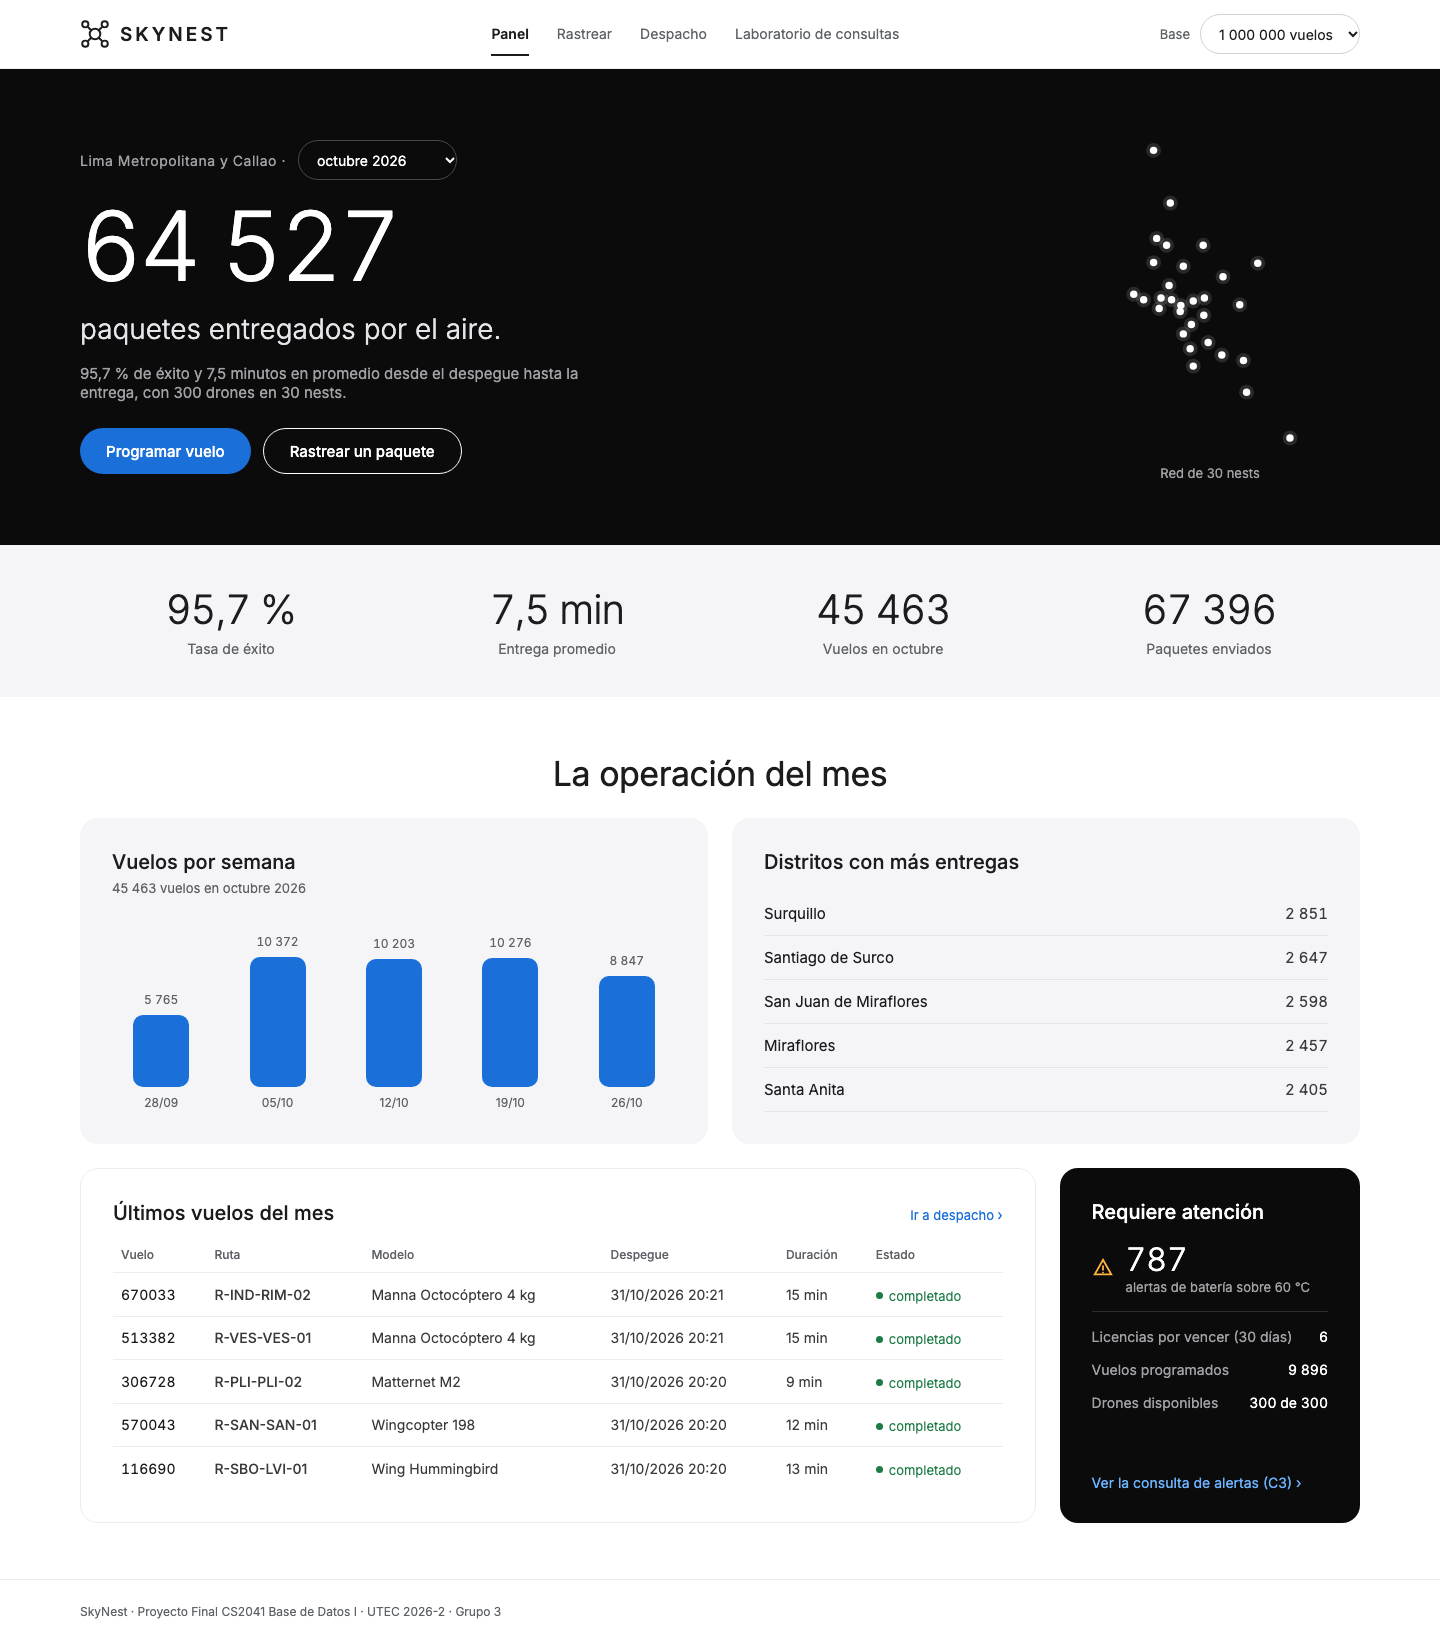
\includegraphics[width=0.85\linewidth,height=0.8\textheight,keepaspectratio]{capturas/01_panel.png}
\caption{Panel con la base de 1\,000\,000 de vuelos (octubre de 2026)}
\end{figure}

\begin{figure}[H]\centering
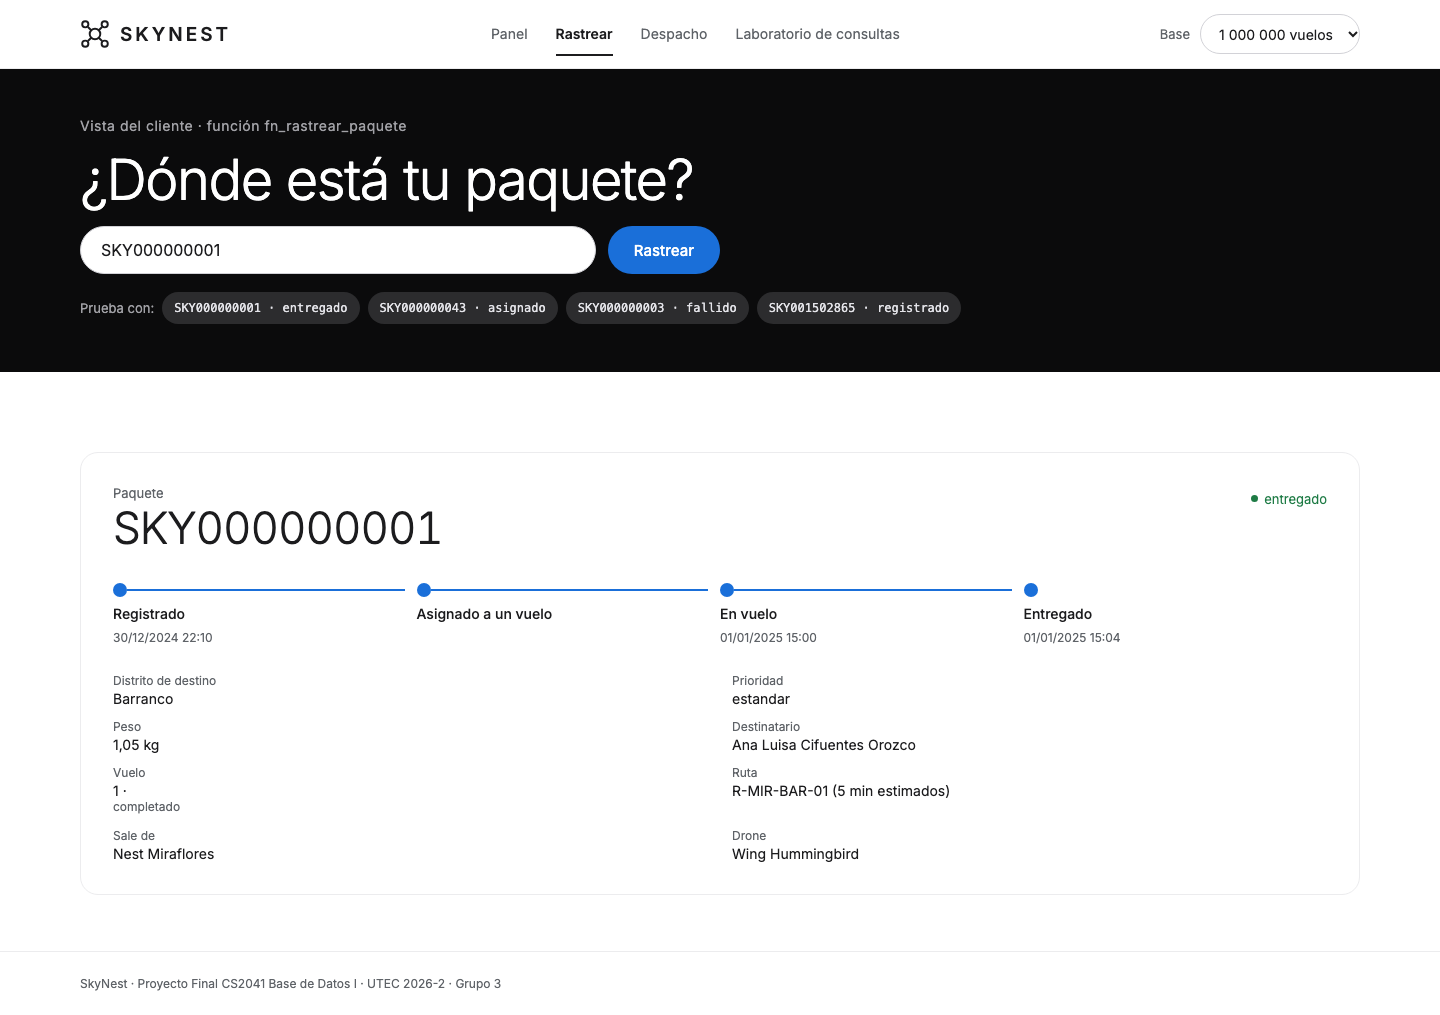
\includegraphics[width=0.85\linewidth,height=0.8\textheight,keepaspectratio]{capturas/02_rastrear.png}
\caption{Rastreo de un paquete con \at{fn\_rastrear\_paquete}}
\end{figure}

\begin{figure}[H]\centering
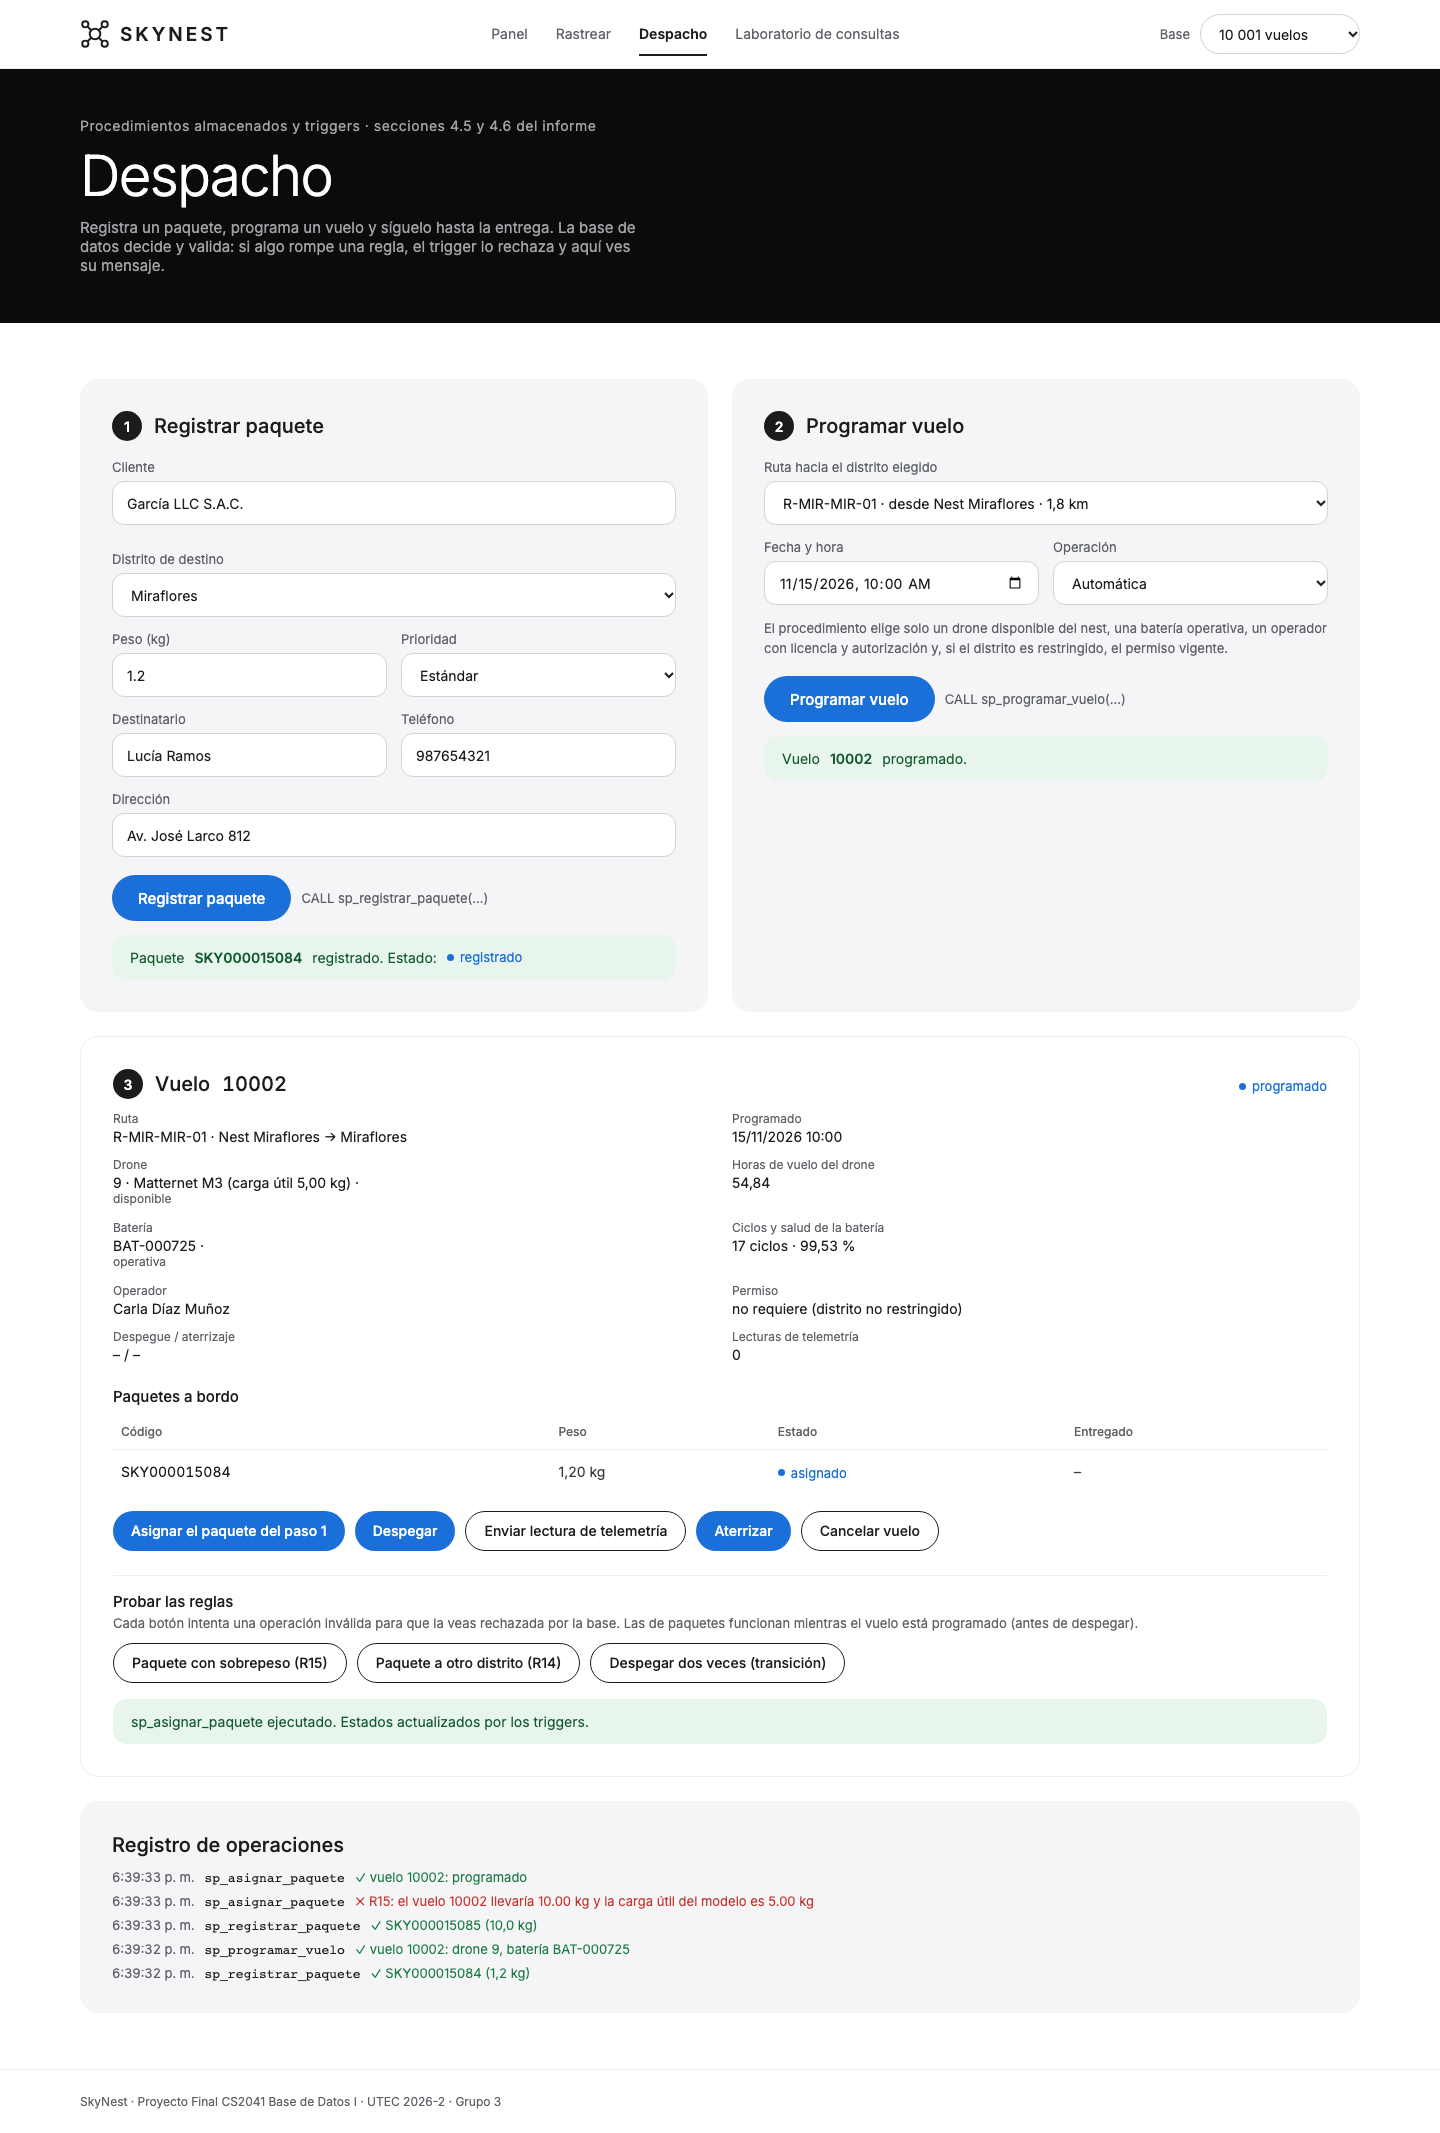
\includegraphics[width=0.85\linewidth,height=0.8\textheight,keepaspectratio]{capturas/03_despacho.png}
\caption{Despacho: paquete registrado, vuelo programado y asignación. En el registro de operaciones se ve el rechazo del trigger de R15 (paquete con sobrepeso).}
\end{figure}

\begin{figure}[H]\centering
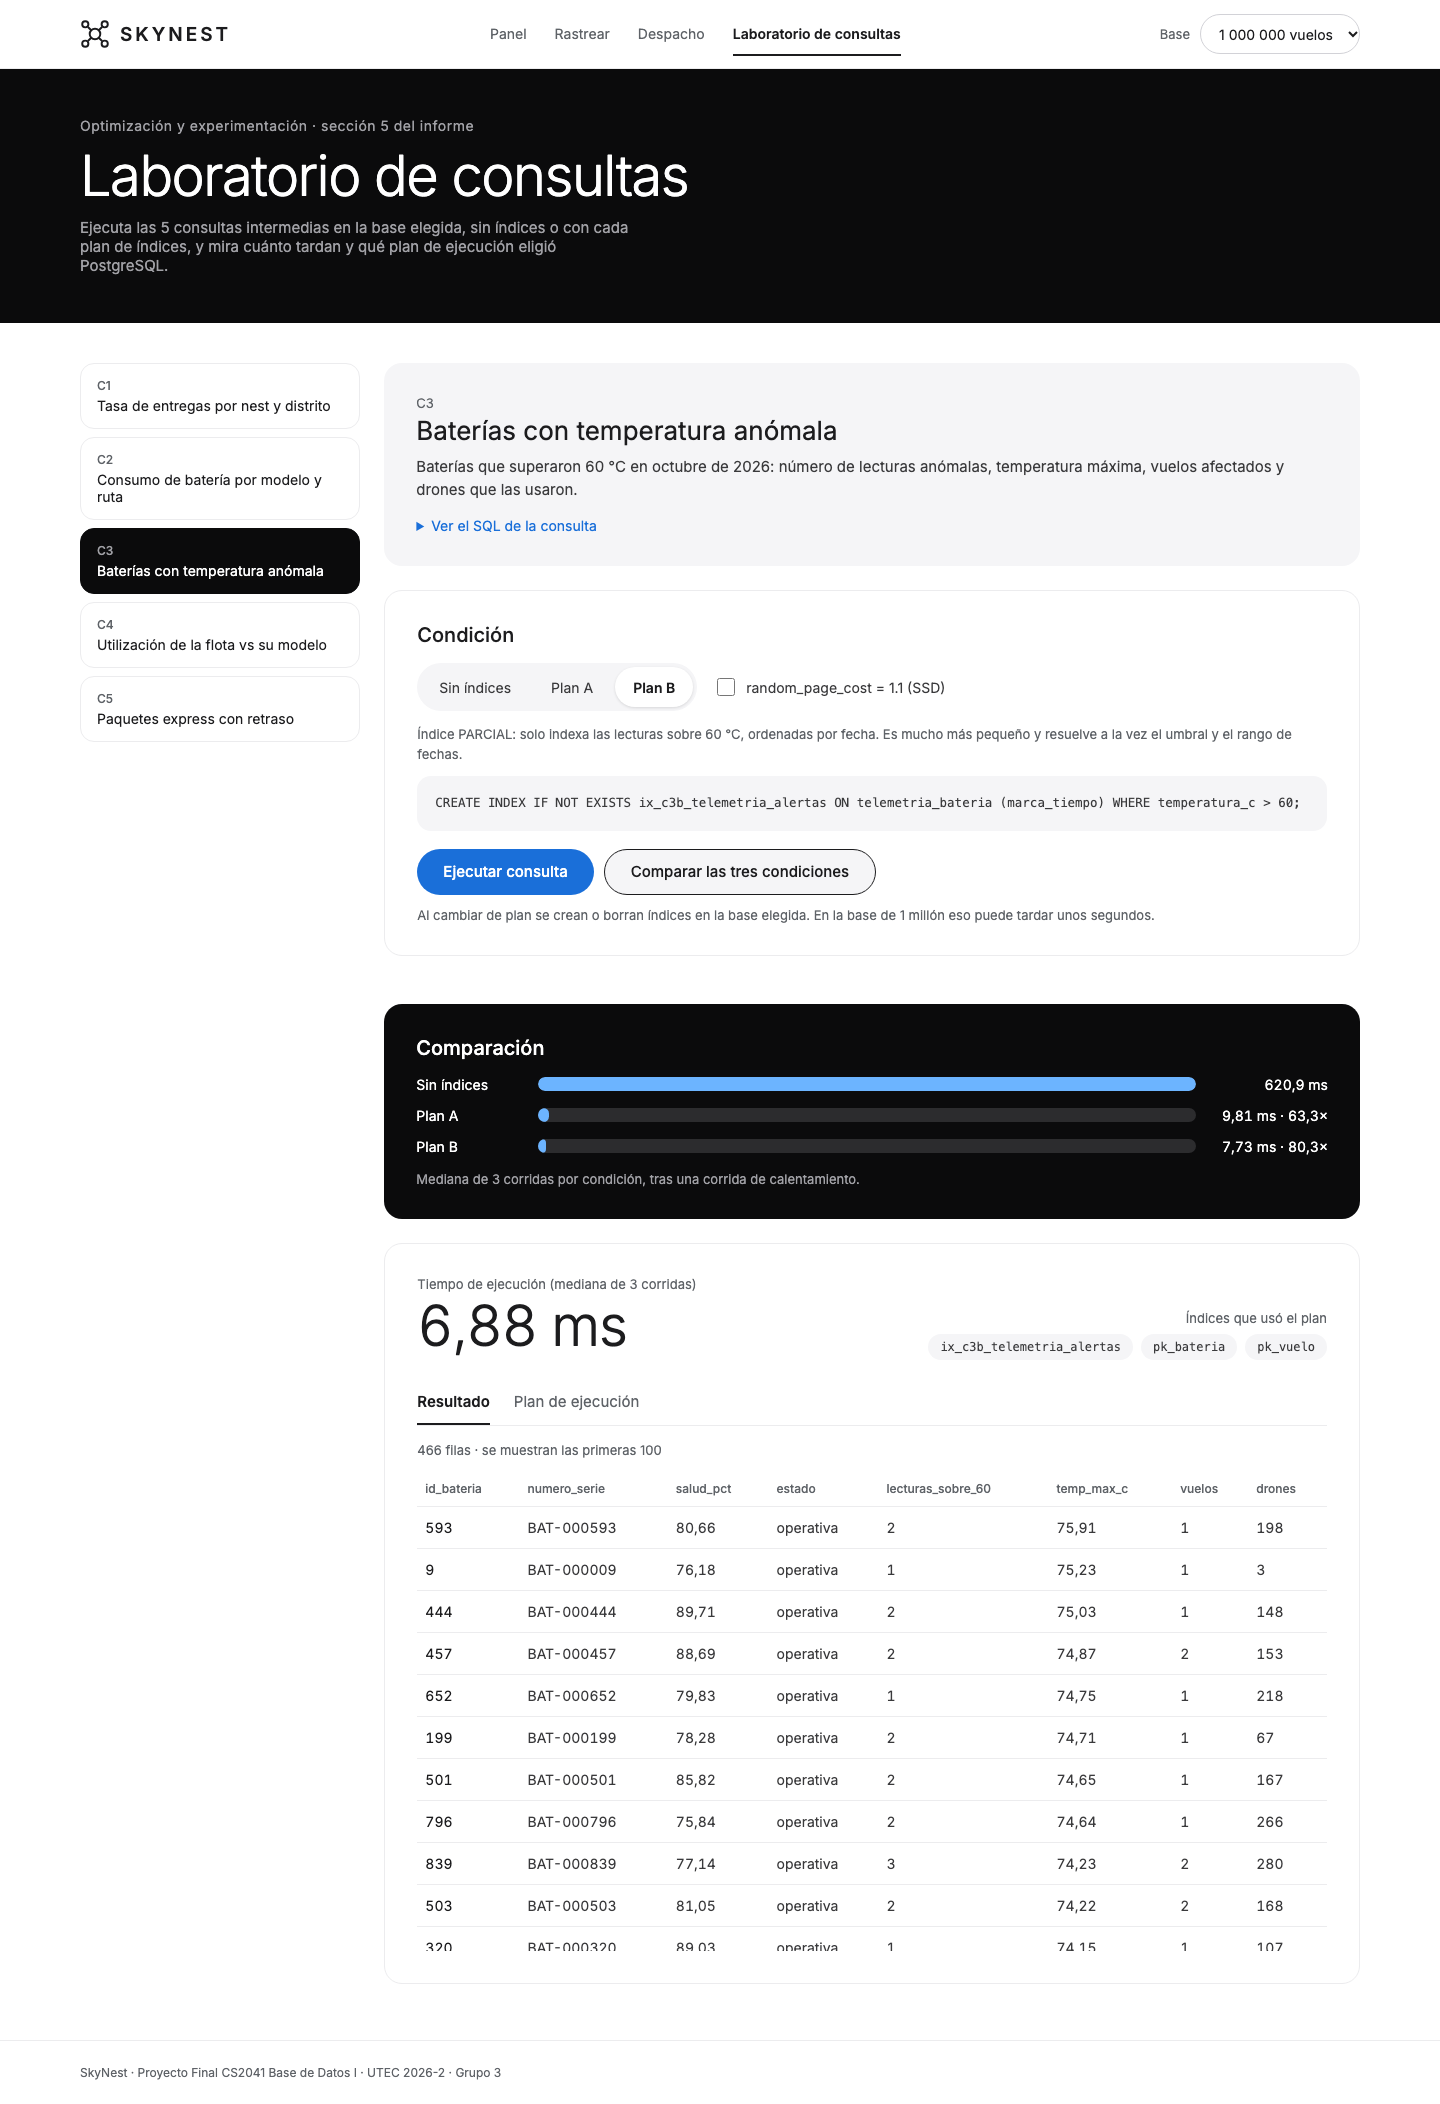
\includegraphics[width=0.85\linewidth,height=0.8\textheight,keepaspectratio]{capturas/04_laboratorio.png}
\caption{Laboratorio: C3 con el plan B y la comparación de las tres condiciones en la base de 1\,000\,000 de vuelos}
\end{figure}

\begin{figure}[H]\centering
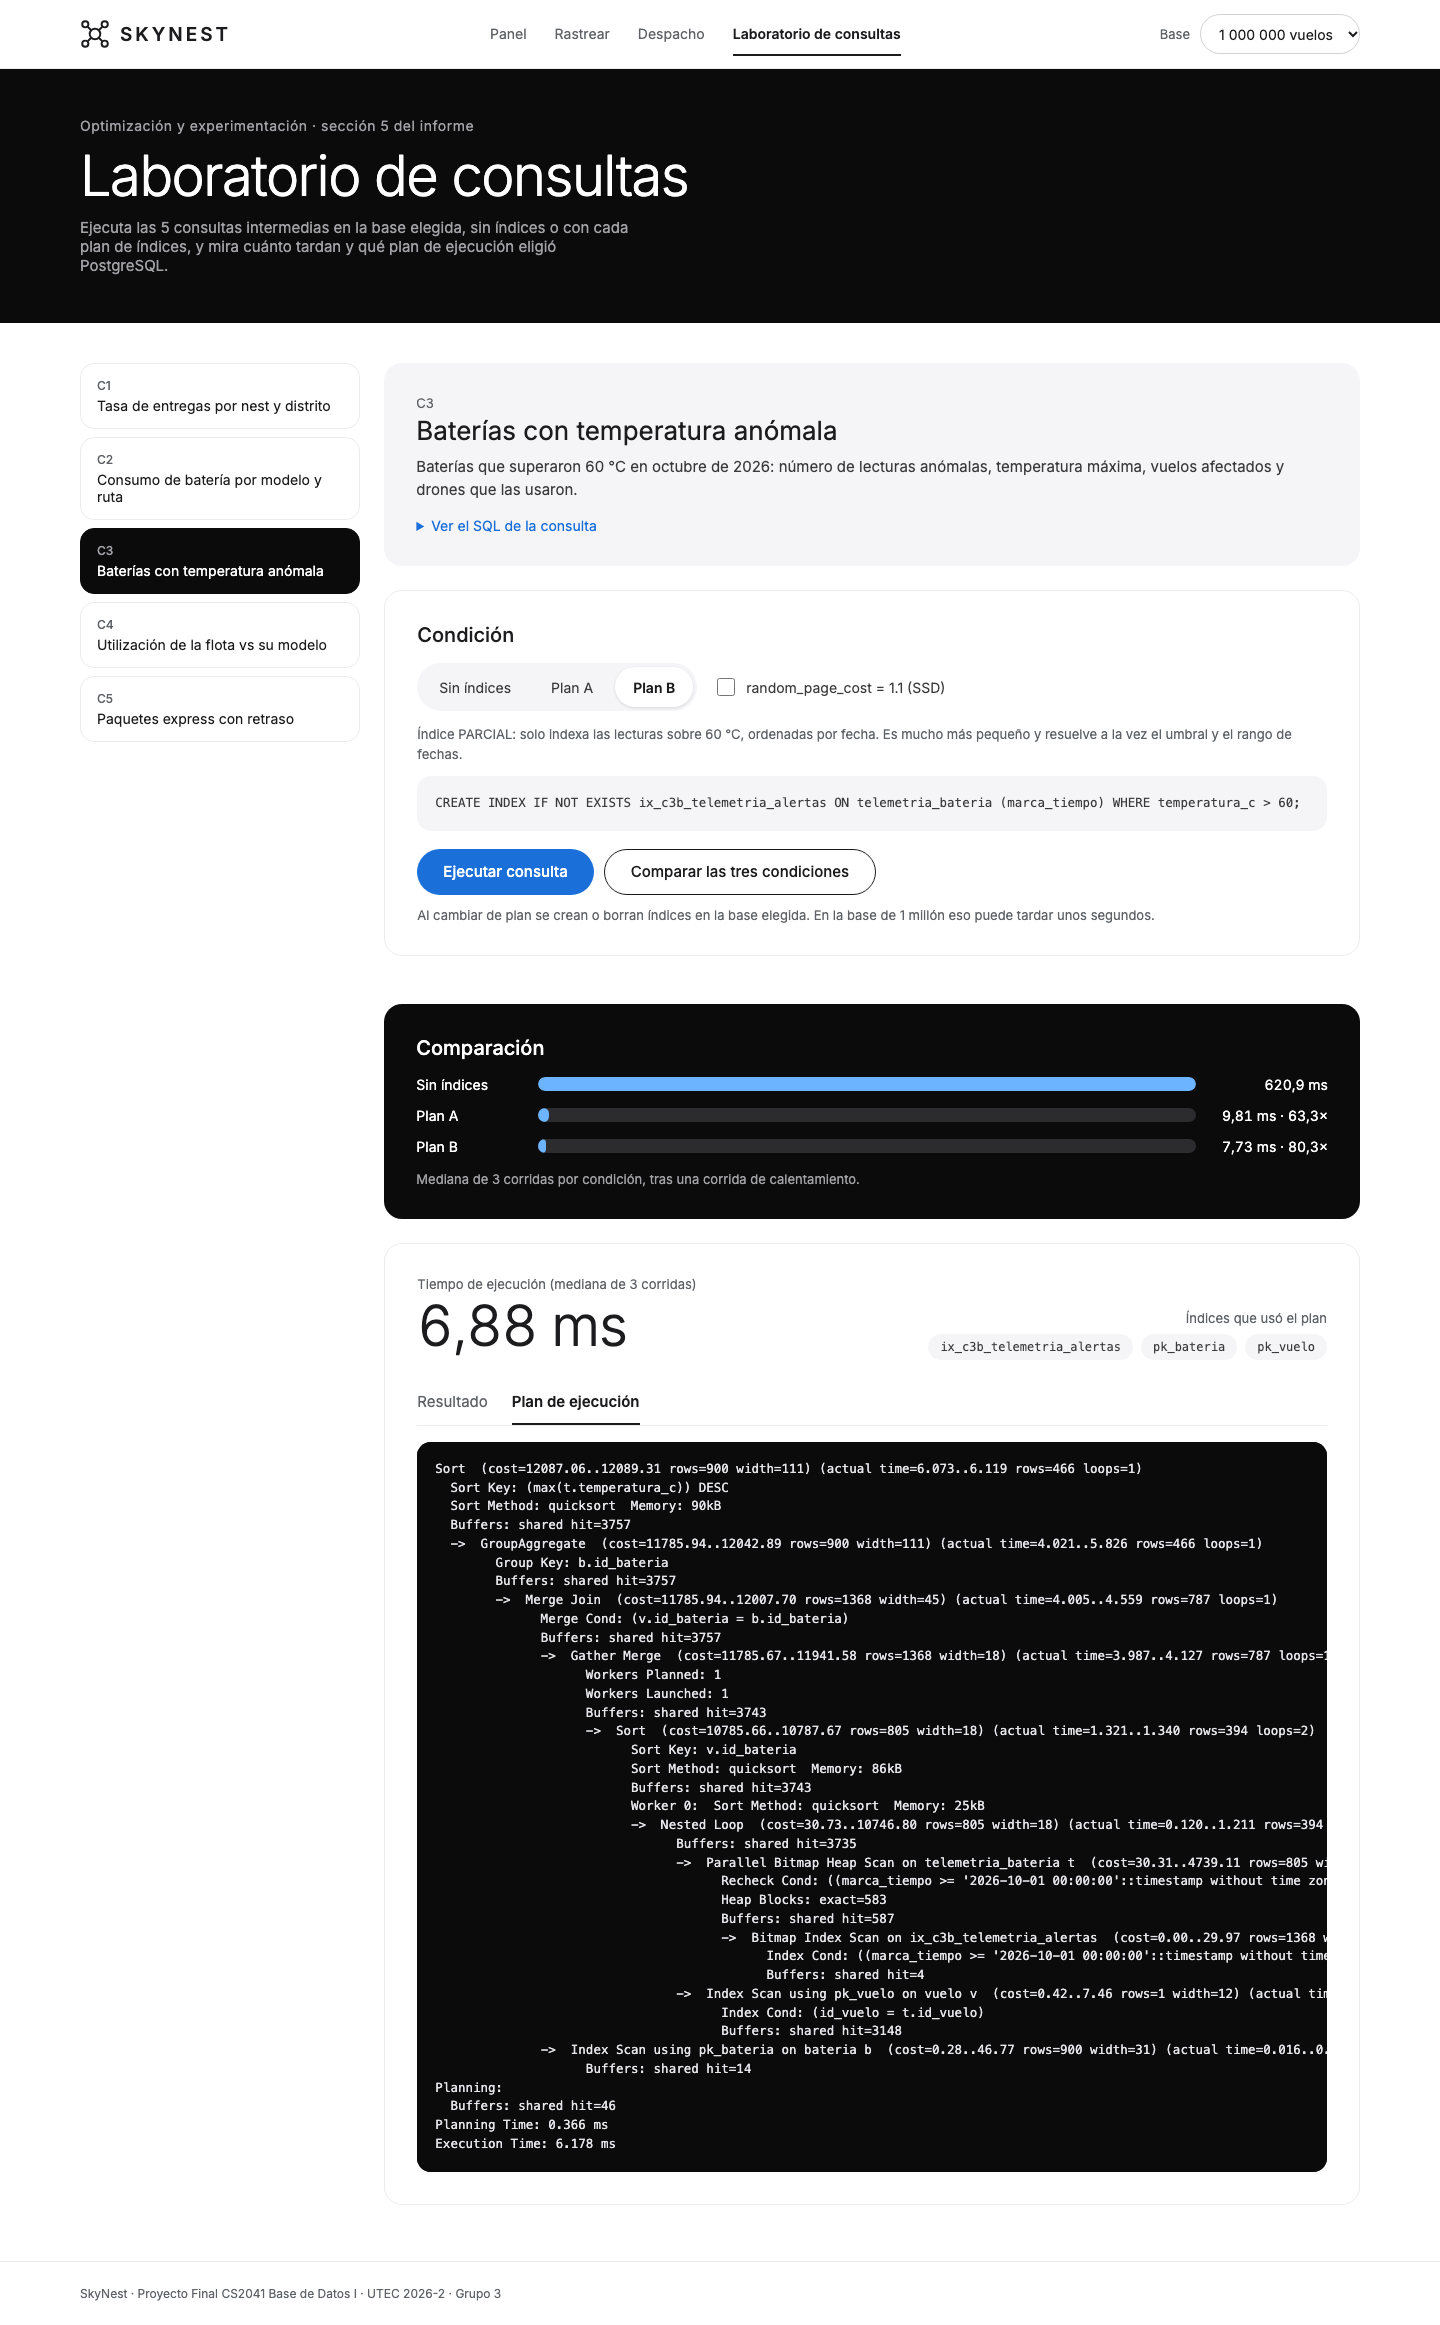
\includegraphics[width=0.85\linewidth,height=0.8\textheight,keepaspectratio]{capturas/05_laboratorio_plan.png}
\caption{Laboratorio: plan de ejecución de C3 con el índice parcial}
\end{figure}

\subsection{Video de la experimentación}
Cinco videos, uno por consulta, ejecutados en pgAdmin sobre la base de 1\,000\,000 de vuelos. Cada uno muestra el plan de ejecución y el tiempo de la consulta sin índices y con el índice que más la mejoró, y al final borra el índice. Los scripts están en \archivo{video_ejemplo/demo_c1.sql} a \archivo{video_ejemplo/demo_c5.sql}.
\begin{itemize}
\item Consulta 1 (índices cubrientes): \url{https://drive.google.com/file/d/1DEceSLNMxklyqunQvqVqOuqCeRu2gj0q/view?usp=sharing}
\item Consulta 2 (índice compuesto): \url{https://drive.google.com/file/d/1Z0WbNbNy_PGJT4Hyp_flKM138V4MB763/view?usp=sharing}
\item Consulta 3 (índice parcial): \url{https://drive.google.com/file/d/1_n6P6XFe2Ad9zzlDHDcNQMmzZyukfyrT/view?usp=sharing}
\item Consulta 4 (B+ en la fecha): \url{https://drive.google.com/file/d/1BN2_Bi6wa98XnyDzW_MDW-j1pnpCZ0Bc/view?usp=sharing}
\item Consulta 5 (compuesto y cubriente, y \texttt{random\_page\_cost = 1.1}): \url{https://drive.google.com/file/d/13Pmu5ubarhSRa7YgPcjhtEzehZe1QTMF/view?usp=sharing}
\end{itemize}

% ---------------------------------------------------------------------
\subsection{Repositorio del proyecto}
\label{sec:repositorio}
Todos los archivos del proyecto están en el repositorio público \url{https://github.com/gdny0208/Proyecto-Final-Skynest}, incluidos los cuatro dumps del experimento (con Git LFS, porque el de 1M supera el límite de 100\,MB por archivo de GitHub). El archivo \archivo{README.md} explica cómo instalarlo, restaurar las bases y repetir el experimento.

\begin{table}[H]
\centering\small
\caption{Contenido del repositorio}
\label{tab:repo}
\begin{tabularx}{\linewidth}{@{}>{\raggedright\arraybackslash}p{4.4cm}>{\raggedright\arraybackslash}X@{}}
\toprule
Carpeta & Contenido \\
\midrule
\archivo{sql/} & scripts 01 a 08 (esquemas y tablas, datos reales, triggers, procedimientos, vistas, roles, consultas e índices) y sus pruebas \\
\archivo{gen/} & generador de datos sintéticos, verificación de las 18 reglas y construcción de las 4 bases \\
\archivo{bench/} & programa del experimento (sección~\ref{sec:metodologia}) \\
\archivo{dumps/} & los 4 dumps: \archivo{skynest_1k.dump} a \archivo{skynest_1m.dump} (Git LFS) \\
\archivo{informe/resultados/} & tiempos de todas las corridas (CSV), los 80 planes de ejecución, gráficos y tablas \\
\archivo{informe/evidencias/} & salidas de la construcción de las bases, las pruebas y el experimento \\
\archivo{video_ejemplo/} & scripts que se ejecutan en los 5 videos (\archivo{demo_c1.sql} a \archivo{demo_c5.sql}) \\
\archivo{web/} & MVP web (FastAPI y PostgreSQL), sección~\ref{sec:mvp} \\
\archivo{docs/} & informe y modelo E/R del Hito 1 \\
\bottomrule
\end{tabularx}
\end{table}

% ---------------------------------------------------------------------
\subsection{Planes de ejecución completos (escala 1M)}
\label{sec:planes_completos}
Salida completa de \texttt{EXPLAIN (ANALYZE, BUFFERS)} de los planes resumidos en la sección~\ref{sec:planes}. Los 80 planes (4 escalas, 5 consultas y 4 condiciones) están en \archivo{informe/resultados/planes/}.

\subsubsection*{Consulta 1}
\textbf{Sin índices:}\plan{1m_C1_sin.txt}
\textbf{Plan B:}\plan{1m_C1_B.txt}
\subsubsection*{Consulta 2}
\textbf{Sin índices:}\plan{1m_C2_sin.txt}
\textbf{Plan A:}\plan{1m_C2_A.txt}
\subsubsection*{Consulta 3}
\textbf{Sin índices:}\plan{1m_C3_sin.txt}
\textbf{Plan B:}\plan{1m_C3_B.txt}
\subsubsection*{Consulta 4}
\textbf{Sin índices:}\plan{1m_C4_sin.txt}
\textbf{Plan A:}\plan{1m_C4_A.txt}
\subsubsection*{Consulta 5}
\textbf{Plan B:}\plan{1m_C5_B.txt}
\textbf{Plan B con \texttt{random\_page\_cost = 1.1}:}\plan{1m_C5_B_rpc.txt}

\subsection{Dumps y scripts}
Los cuatro dumps (\archivo{skynest_1k.dump}, \archivo{skynest_10k.dump}, \archivo{skynest_100k.dump} y \archivo{skynest_1m.dump}) están en la carpeta \archivo{dumps/} del repositorio (sección~\ref{sec:repositorio}). Se descargan desde la web de GitHub (botón \emph{Download} de cada archivo, \url{https://github.com/gdny0208/Proyecto-Final-Skynest/tree/main/dumps}) o, después de clonar el repositorio, con \texttt{git lfs pull}. Se restauran con:
\begin{lstlisting}[style=salida]
createdb skynest_1m && pg_restore -d skynest_1m dumps/skynest_1m.dump
psql -d skynest_1m -c "ALTER DATABASE skynest_1m SET search_path = skynest, reportes, public"
\end{lstlisting}
La segunda línea se necesita porque \texttt{pg\_dump} guarda los esquemas y su contenido, pero no la ruta de búsqueda por defecto de la base.
Para reconstruir todo desde cero (bases, verificación, dumps) y repetir el experimento:
\begin{lstlisting}[style=salida]
bash gen/construir_bases.sh                  # 4 bases + 4 dumps
.venv/bin/python bench/experimento.py        # tablas, gráficos y planes en informe/resultados/
\end{lstlisting}
